\section{Funktionen \& Eigenschaften}

Unter Funktionen verstehen wir Relationen mit dem Unterschied, dass wir die folgende Zusatzbedingung fordern: Zu jedem \( x \) wird \textbf{genau ein} \( y \) zugeordnet.

\subsection{Ganzrationale Funktionen}

\subsubsection{Konstante Funktion}

\[
    y = c
\]

\begin{figure}[H]
    \centering
    \begin{tikzpicture}
        \begin{axis}[
            defaultnonumbers,
            xmin=-4.2, xmax=4.2,
            ymin=-4.2, ymax=4.2,
            width=4.4cm
            ]
            \draw [orange] plot (\x, {3});
            \node at (axis cs: -2/3, 3) {\( c \)};
            \draw[-] (-0.25,3) -- (0.25,3);
        \end{axis}
    \end{tikzpicture}
\end{figure}

\subsubsection{Lineare Funktion}

\[
    y = \underbrace{m x}_{\text{Steigung}} + n
\]

\begin{figure}[H]
    \centering
    \begin{tikzpicture}
        \begin{axis}[
            defaultnonumbers,
            xmin=-4.2, xmax=4.2,
            ymin=-4.2, ymax=4.2,
            width=4.4cm
            ]
            \draw [orange] plot (\x, {2 * \x + 1});
            \node at (axis cs: -2/3, 1) {\( n \)};
            \draw[-] (-0.25,1) -- (0.25,1);
        \end{axis}
    \end{tikzpicture}
\end{figure}

\subsubsection{Quadratische Funktion}

\[
	y = \underbrace{\underbrace{ax^2}_{\text{Potenzfunktion}} + bx + c}
	_{\text{Polynom / ganze Funktion}}
\]

\begin{figure}[H]
	\centering
	\begin{tikzpicture}
		\begin{axis}[
				defaultnonumbers,
				xmin=-2.2, xmax=6.2,
				ymin=-2.2, ymax=6.2,
				width=8.8cm
			]
			\draw [cyan, smooth, samples=100] plot (\x, {pow(\x, 2)});
			\draw [color1, smooth, samples=100] plot (\x, {pow(\x, 2) - 6 * \x + 11});
			\node at (axis cs: -2/3, 2) {\( b \)};
			\node at (axis cs: -2/3, 3) {\( y_0 \)};
			\node at (axis cs: 3, -2/3) {\( a \)};
			\node at (axis cs: 4, -2/3) {\( x_0 \)};
			\draw[-, gray] (0,2) -- (3,2);
			\draw[-, gray] (0,3) -- (4,3);
			\draw[-, gray] (3,0) -- (3,2);
			\draw[-, gray] (4,0) -- (4,3);
		\end{axis}
	\end{tikzpicture}
\end{figure}

\begin{align*}
	y         & = x^2               & \rightarrow y'   & = x'^2    \\
	x_0       & = a + x'_0          & \Rightarrow x'_0 & = x_0 - a \\
	y_0       & = b + y'_0          & \Rightarrow y'_0 & = y_0 - b \\
	\\
	y'        & = x'^2                                             \\
	(y_0 - b) & = {(x_0 -a)}^2                                     \\
	y_0       & = {(x_0 - a)}^2 + b                                \\
	y         & = {(x - a)}^2 + b
\end{align*}

\paragraph{Verschiebung auf der x-Achse}

\begin{description}[style=nextline]
	\item[negatives \(a\)] Verschiebung nach rechts
	\item[positives \(a\)] Verschiebung nach links
\end{description}

\paragraph{Herleitung der p-q-Formel}

\begin{align*}
	                &  & y = a x^2 + b x +c                      & = 0                                                                                             \\
	\\
	                &  & x^2 + px + q                            & = 0                                                                                             \\
	\Leftrightarrow &  & x^2 + px                                & = -q                                                       & \mid \text{Quadratische Ergänzung} \\
	\Leftrightarrow &  & x^2 + px + {\left(\frac{p}{2}\right)}^2 & = -q + {\left(\frac{p}{2}\right)}^2                                                             \\
	\Leftrightarrow &  & {\left( x+\frac{p}{2} \right)}^2        & = {\left(\frac{p}{2}\right)}^2 - q                                                              \\
	\Rightarrow     &  & x + \frac{p}{2}                         & = \pm \sqrt{{\left(\frac{p}{2}\right)}^2 - q}                                                   \\
	\Leftrightarrow &  & x_{1,2}                                 & = -\frac{p}{2} \pm \sqrt{{\left(\frac{p}{2}\right)}^2 - q}
\end{align*}


\subsubsection{Kubische Funktion}

\[
	y = f(x) = c_1 x^3 + c_2 x^2 + c_3 x + c_4
\]

\begin{figure}[H]
	\centering
	\begin{tikzpicture}
		\begin{axis}[
				defaultnonumbers,
				xmin=-4.2, xmax=4.2,
				ymin=-4.2, ymax=4.2,
				width=4.4cm
			]
			\draw [orange, smooth, samples=100] plot (\x, {pow(\x, 3)});
		\end{axis}
	\end{tikzpicture}
\end{figure}

\subsection{Symmetrie}

\subsubsection{Achsensymmetrie}

\[
    f(-x) = f(x)  
\]

Ist der Fall für jede \enquote{gerade Funktion}, d.h.\ eine Funktion mit
ausschließlich geraden Exponetenten.

\begin{figure}[H]
    \centering
    \begin{tikzpicture}
        \begin{axis}[
            defaultnonumbers,
            xmin=-4.2, xmax=4.2,
            ymin=-2.2, ymax=6.2,
            width=6cm
            ]
            \addplot[orange, smooth, samples=100] {x^2};
            \draw[dotted, thick] (2,0) -- (2,4);
            \draw[dotted, thick] (-2,0) -- (-2,4);
            \draw[dotted, thick] (-2,4) -- (2,4);
            \node at (axis cs: 2, -2/3) {\( x_0 \)};
            \node at (axis cs: -2, -2/3) {\( -x_0 \)};
            \node at (axis cs: -2/3, 4 + 2/3) {\( y_0 \)};
        \end{axis}
    \end{tikzpicture}
    \caption{Achsensymmetrie}\label{fig:achsensymmetrie}
\end{figure}

\subsubsection{Punktsymmetrie (zum Ursprung)}

\[
    f(-x) = -f(x)  
\]

Ist der Fall für jede \enquote{ungerade Funktion}, d.h.\ eine Funktion mit
ausschließlich ungeraden Exponetenten.

\begin{figure}[H]
    \centering
    \begin{tikzpicture}
        \begin{axis}[
            defaultnonumbers,
            xmin=-4.2, xmax=4.2,
            ymin=-4.2, ymax=4.2,
            width=6cm
            ]
            \draw[orange, smooth, samples=100] plot (\x, {pow(\x, 3)});
            \draw[dotted, thick] (1.5,0) -- (1.5,27/8);
            \draw[dotted, thick] (-1.5,0) -- (-1.5,-27/8);
            \draw[dotted, thick] (0,27/8) -- (1.5,27/8);
            \draw[dotted, thick] (0,-27/8) -- (-1.5,-27/8);
            \node at (axis cs: 1.5, -2/3) {\( x_0 \)};
            \node at (axis cs: -1.5, 2/3) {\( -x_0 \)};
            \node at (axis cs: -2/3, 27/8) {\( y_0 \)};
            \node at (axis cs: 2/3, -27/8) {\( -y_0 \)};
        \end{axis}
    \end{tikzpicture}
    \caption{Punktsymmetrie}\label{fig:punktsymmetrie}
\end{figure}

\subsubsection{Symmetrie bei gebrochenen Funktionen}

\begin{align*}
    f(x) &= \frac{\text{gerade}}{\text{ungerade}} &&\hat{=}\ \text{ungerade Funktion} \\
    f(x) &= \frac{\text{ungerade}}{\text{gerade}} &&\hat{=}\ \text{ungerade Funktion} \\
    f(x) &= \frac{\text{gerade}}{\text{gerade}} &&\hat{=}\ \text{gerade Funktion} \\
    f(x) &= \frac{\text{ungerade}}{\text{ungerade}} &&\hat{=}\ \text{gerade Funktion}
\end{align*}

\subsubsection{Beispiele}

\begin{align*}
    y = f(x) &= x^2 + 2x - 5 \\
    f(-x) &= {(-x)}^2 + 2(-x) - 5 = x^2 - 2x - 5 &&\rightarrow \text{keine Achsensymmetrie} \\
    -f(x) &= -1(x^2 + 2x - 5) = x^2 - 2x +5 &&\rightarrow \text{keine Punktsymmetrie}
\end{align*}

\textit{\(f(x)\) ist weder gerade noch ungerade, somit kann man auch direkt sehen,
    dass die Funktion nicht symmetrisch ist.}


\[
    f(x) = x^7 + 3x^3 \rightarrow \text{punktsymmetrisch, da ungerade}
\]

\[
    \begin{array}{lll}
        y = \sqrt{x^2 - 25}   &\rightarrow \text{gerade Funktion} &\rightarrow \text{Achsensymmetrie} \\
        y = \sin(x) - \cos(x) &\rightarrow \text{ungerade Funktion} &\rightarrow \text{Punktsymmetrie} \\
        & \quad\text{(\(\sin(x)\) ist ungerade)} & \\
        y = 4 \cdot \sin^2(x) &\rightarrow \text{gerade Funktion} &\rightarrow \text{Achsensymmetrie}
    \end{array}        
\]

\subsubsection{Symmetrie zur Quadrantenhalbierenden}

\begin{figure}[H]
    \centering
    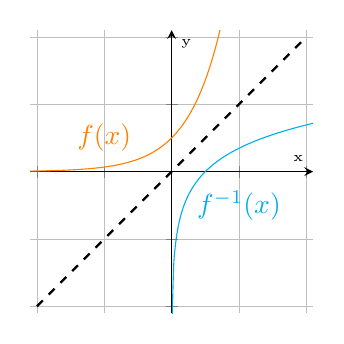
\begin{tikzpicture}
        \begin{axis}[
            unit vector ratio*=1 1 1,
            xmin=-4.2, xmax=4.2,
            ymin=-4.2, ymax=4.2,
            width=6cm,
            grid=both,
            axis lines=middle,
            grid style={line width=.1pt, draw=gray!20},
            major grid style={line width=.2pt,draw=gray!50},    
            ticklabel style={font=\tiny},
            xticklabels={,,},
            yticklabels={,,},
            xlabel style={font=\tiny},
            ylabel style={font=\tiny},
            xlabel={x}, ylabel={y}
            ]
            \draw [orange, smooth, samples=100] plot (\x, {exp(\x)});
            \draw [cyan, smooth, samples=100, domain=1/100:5] plot (\x,
            {ln(\x)});
            \draw[dashed, thick] (-4,-4) -- (4,4);
            \node[orange] at (axis cs: -2, 1) {\( f(x) \)};
            \node[cyan] at (axis cs: 2, -1) {\( f^{-1}(x) \)};
        \end{axis}
    \end{tikzpicture}
    \caption{Symmetrie zur Quadrantenhalbierenden}\label{fig:symquadrantenhalbierende}
\end{figure}

\subsubsection{Umkehrfunktion}

\[
    f^{-1}(x) \neq \frac{1}{f(x)}
\]

\(^{-1}\) steht für die Umkehrfunktion und nicht für eine \(-1\) im Exponenten.

\begin{figure}[H]
    \centering
    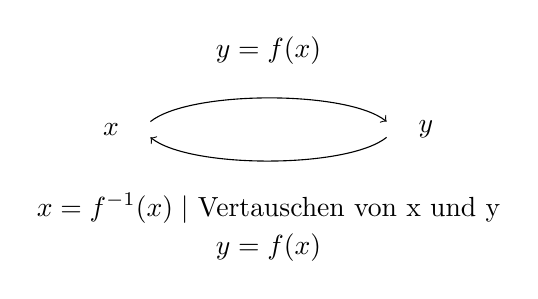
\begin{tikzpicture}
      \node at (-2,0) {\(x\)};
      \node at (2,0) {\(y\)};
      \draw[->] (-1.5,0.1) .. controls (-1,0.5) and (1,0.5) .. (1.5,0.1);
      \draw[<-] (-1.5,-0.1) .. controls (-1,-0.5) and (1,-0.5) .. (1.5,-0.1);
      \node at (0, 1) {\(y = f(x)\)};
      \node at (0, -1) {\(x = f^{-1}(x) \mid \) Vertauschen von x und y};
      \node at (0, -1.5) {\(y=f(x)\)};
    \end{tikzpicture}
\end{figure}

\begin{align*}
    f &= \{ (x,y) \mid x \in D_f, y \in W_f, y = f(x) \} \\
    f^{-1} &= \{ (y,x) \mid y \in D_f^{-1} = W_f, x \in W_f^{-1}, x = f^{-1}(y) \} \\
    \Rightarrow f^{-1} &= \{ (x,y) \mid x \in D_f^{-1} = W_f, y \in W_f^{-1}, y = f^{-1}(x) \}
\end{align*}

\paragraph{Rechenrezept}

\begin{itemize}
    \item \(x\) und \(y\) vertauschen
    \item \(x = f(y)\) nach \(y\) auflösen
\end{itemize}

\paragraph{Beispiel}

\begin{align*}
    y &= f(x) = 2x - 1 \\
    x &= 2y - 1 \\
    y &= \frac{x + 1}{2}
\end{align*}

\begin{figure}[H]
    \centering
    \begin{tikzpicture}
        \begin{axis}[
            defaultnonumbers,
            xmin=-4.2, xmax=4.2,
            ymin=-4.2, ymax=4.2,
            width=4.4cm
            ]
            \draw[orange] plot (\x, {2 * \x - 1});
            \draw[cyan] plot (\x, {(\x + 1) / 2 });
            \draw[dashed] (-4,-4) -- (4,4);
            \node[orange] at (axis cs: 2, -1) {\( f(x) \)};
            \node[cyan] at (axis cs: -2, 1) {\( f^{-1}(x) \)};
        \end{axis}
    \end{tikzpicture}
\end{figure}

% BILD
% x^2 und sqrt(x)

\paragraph{Beispiele}

\subparagraph{1. Beispiel (siehe Abb.~\ref{fig:beispiel1_umkehrfunktion})}

\begin{align*}
    y = f(x) &= \frac{5x}{x+1} -2 \\
    x &= \frac{5y}{y+1} -2 &&\mid +2 \\
    x+2 &= \frac{5y}{y+1} &&\mid  \cdot (y + 1) \\
    (x+2)(x+1) &= 5y \\
    xy + x + 2y + 2 &= 5y &&\mid -xy-2y \\
    x + 2 &= 5y -xy -2y \\
    x + 2 &= y (5-x -2 ) &&\mid : (2-x) \\
    y &= \frac{x+2}{3-x} = f^{-1}(x)
\end{align*}

\begin{figure}[H]
    \centering
    \begin{tikzpicture}
        \begin{axis}[
            defaultnonumbers,
            xmin=-10.2, xmax=10.2,
            ymin=-10.2, ymax=10.2,
            width=6.4cm
            ]
            \draw[orange, smooth, samples=100, domain=-10:-1-1/10] plot (\x, {(5*\x)/(\x + 1)-2});
            \draw[orange, smooth, samples=100, domain=-1+1/10:10] plot (\x, {(5*\x)/(\x + 1)-2});
            \draw[cyan, smooth, samples=100, domain=-10:3-1/10] plot (\x, {(\x + 2) / (3 - \x) });
            \draw[cyan, smooth, samples=100, domain=3+1/10:10] plot (\x, {(\x + 2) / (3 - \x) });
            \draw[dashed] (-10,-10) -- (10,10);
        \end{axis}
    \end{tikzpicture}
    \caption{orange: \(f(x)\), cyan: \(f^{-1}(x)\)}\label{fig:beispiel1_umkehrfunktion}
\end{figure}

\subparagraph{2. Beispiel (siehe Abb.~\ref{fig:beispiel2_umkehrfunktion})}

\begin{align*}
    y = f(x) &= \frac{x+1}{x-1} \\
    x &= \frac{y+1}{y-1} &&\mid \cdot (y-1) \\
    x(y-1) &= y+1 &&\mid -1 \\
    y &= x(y-1)-1 \\
    y &= xy - x - 1 &&\mid -xy \\
    y - xy &= -x - 1 \\
    y(1-x) &= -x -y &&\mid : (1-x) \\
    y &= \frac{-x-1}{1-x} \\
    y &= \frac{-x-1}{1-x} \\
    y &= \frac{-1(x+1)}{1-x} \\
    y &= -1 \frac{x+1}{1-x} \\
    y &= \frac{x+1}{-1(1-x)} \\
    y &= \frac{x+1}{x-1} = f^{-1}(x)
\end{align*}

\begin{figure}[H]
    \centering
    \begin{tikzpicture}
        \begin{axis}[
            defaultnonumbers,
            xmin=-10.2, xmax=10.2,
            ymin=-10.2, ymax=10.2,
            width=6.4cm
            ]
            \draw[orange, smooth, samples=100, domain=-10:1-1/10] plot (\x,
            {(\x + 1)/(\x - 1)});
            \draw[orange, smooth, samples=100, domain=1+1/10:10] plot (\x,
            {(\x + 1)/(\x - 1)});
            \draw[cyan, dashed, smooth, samples=100, domain=-10:1-1/10] plot (\x,
            {(\x + 1)/(\x - 1)});
            \draw[cyan, dashed, smooth, samples=100, domain=1+1/10:10] plot (\x,
            {(\x + 1)/(\x - 1)});
            \draw[dashed] (-10,-10) -- (10,10);
        \end{axis}
    \end{tikzpicture}
    \caption{orange: \(f(x)\), cyan: \(f^{-1}(x)\) (liegen aufeinander)}\label{fig:beispiel2_umkehrfunktion}
\end{figure}

\subparagraph{3. Beispiel (siehe Abb.~\ref{fig:beispiel3_umkehrfunktion})}

\begin{align*}
    y &= f(x) = F(\phi(x)) \\
    x &= F(\phi(y)) &&\mid F^{-1} \\
    F^{-1}(x) &= \phi(y) &&\mid \phi^{-1} \\
    \phi^{-1}(F^{-1}(x)) &= y = f^{-1}(x)
\end{align*}

\begin{figure}[H]
    \centering
    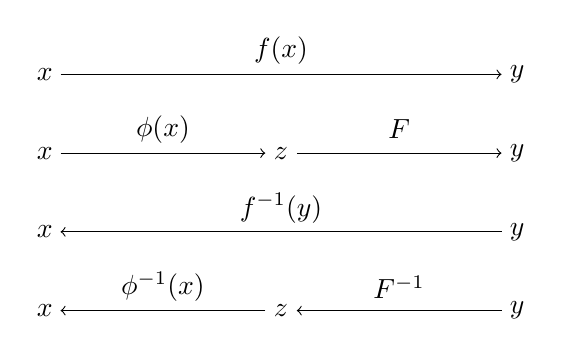
\begin{tikzpicture}
      \node[] at (0, 0) {\(x\)};
      \node[] at (0,-1) {\(x\)};
      \node[] at (0,-2) {\(x\)};
      \node[] at (0,-3) {\(x\)};

      \node[] at (6, 0) {\(y\)};
      \node[] at (6,-1) {\(y\)};
      \node[] at (6,-2) {\(y\)};
      \node[] at (6,-3) {\(y\)};

      \node[] at (3,-1) {\(z\)};
      \node[] at (3,-3) {\(z\)};
      
      \node[] at (3,   0.3) {\(f(x)\)};
      \node[] at (1.5,-0.7) {\(\phi(x)\)};
      \node[] at (4.5,-0.7) {\(F\)};
      \node[] at (3,  -1.7) {\(f^{-1}(y)\)};
      \node[] at (1.5,-2.7) {\(\phi^{-1}(x)\)};
      \node[] at (4.5,-2.7) {\(F^{-1}\)};
      
      \draw[->] (0.2, 0) -- (5.8, 0);
      \draw[->] (0.2,-1) -- (2.8,-1);
      \draw[->] (3.2,-1) -- (5.8,-1);
      \draw[->] (5.8,-2) -- (0.2,-2);
      \draw[->] (2.8,-3) -- (0.2,-3);
      \draw[->] (5.8,-3) -- (3.2,-3);
    \end{tikzpicture}
    \caption{Grafische Darstellungsform}\label{fig:beispiel3_umkehrfunktion}
  \end{figure}


\subsection{Nullstellen}

\subsubsection{Beispiele}

\paragraph{1. Beispiel}

\[
	f(x) = 9x^2-x^4
\]

\begin{figure}[H]
	\centering
	\begin{tikzpicture}
		\begin{axis}[
				defaultpure,
				xmin=-4.2, xmax=4.2,
				ymin=-2.2, ymax=22.2,
				width=6cm
			]
			\draw [orange, smooth, samples=100, domain=-4:4] plot (\x, {9 * pow(\x, 2) -
					pow(\x, 4)});
		\end{axis}
	\end{tikzpicture}
	\caption{\(f(x) = 9x^2-x^4\)}\label{fig:nullstellen_grad4}
\end{figure}


\begin{align*}
	D_f = \{ x \mid x \in \mathbb{R} \}       \\
	\text{Symmetrie:} f(x) \text{ ist gerade} \\
	-x^4 \rightarrow \text{geht ins negative} \\
	\lim_{x\rightarrow\pm\infty} = - \infty
\end{align*}

Nullstellen:

\[
	f(x) = x^2(9-x^2) = x^2 (3^2 - x^2) = \underbrace{x^2}_{0\ \text{(doppelt)}} (3 - \underbrace{x}_{3}) (3 + \underbrace{x}_{-3})
\]

\paragraph{2. Beispiel}

\[
	f(x) = (x^2 - 1)(x^2 - 4) x
\]

\begin{figure}[H]
	\centering
	\begin{tikzpicture}
		\begin{axis}[
				default,
				xmin=-4.2, xmax=4.2,
				ymin=-4.2, ymax=4.2,
				width=6cm
			]
			\draw [orange, smooth, samples=100, domain=-2.5:2.5] plot (\x, {(pow(\x,
					2) - 1) * (pow(\x, 2) - 4) * \x});
		\end{axis}
	\end{tikzpicture}
	\caption{\(f(x) = (x^2 - 1)(x^2 - 4)x\)}\label{fig:nullstellen_grad5}
\end{figure}

\begin{align*}
	f(x) & = \underbrace{(x^2-1)}_{x = \pm 1}
	\underbrace{(x^2-4)}_{x = \pm 2}
	\underbrace{x}_{x = 0}                    \\
	     & = (x^4 - x^2 - 4x^2 + 4)x          \\
	     & = x^5 - x^3 - 4x^3 +4x             \\
	     & = x^5 - 5x^3 + 4x
\end{align*}

\begin{align*}
	\limtoinfty{x} f(x)    & = \infty  \\
	\limtomininfty{x} f(x) & = -\infty
\end{align*}

\begin{itemize}
	\item ungerade Exponenten: punktsymetrisch zum Ursprung
	\item Höchster Exponent:5 \\
	      \textrightarrow\ Funktion 5. Grades \\
	      \textrightarrow\ 5 Nullstellen
\end{itemize}



\subsection{Gebrochen rationale Funktionen}

\[
    y = f(x) = \frac{a_0 + a_1 x^1 + a_2 x^2 + \cdots + a_z x^z}
    {b_0 + b_1 x^1 + b_2 x^2 + \cdots + b_z x^n}
    = \frac{\sum_{i=0}^{z} a_i\ x^i}{\sum_{i=0}^{n} b_i\ x^i}
\]

für \(n > 0\) und \(z < n\): echt gebrochen

für \(n > 0\) und \(z \geq n\): unecht gebrochen

\paragraph{Unecht gebrochene Funktionen}

\[
    G(x) = \frac{Z(x)}{N(x)} = \underbrace{S(x)}_{\text{ganze Fkt.}} + \underbrace{\frac{R(x)}{N(x)}}_{\text{echt gebrochen}}
\]

\subsubsection{Beispiele}

\paragraph{1. Beispiel (einfachste gebrochene Funktion) (siehe Abb.~\ref{fig:gebrochenefunktionen_beispiel1})}

\[
    y = f(x) = \frac{1}{x}  
\]

punktsymmetrisch

\begin{figure}[H]
    \centering
    \begin{tikzpicture}
        \begin{axis}[
            default,
            xmin=-4.2, xmax=4.2,
            ymin=-4.2, ymax=4.2,
            width=6cm
            ]
            \draw [orange, smooth, samples=100, domain=-4:-1/100] plot (\x, {1 / \x});
            \draw [orange, smooth, samples=100, domain=1/100:4] plot (\x, {1 / \x});
        \end{axis}
    \end{tikzpicture}
    \caption{\(f(x) = \frac{1}{x}\)}\label{fig:gebrochenefunktionen_beispiel1}
\end{figure}

\paragraph{2. Beispiel  (siehe Abb.~\ref{fig:gebrochenefunktionen_beispiel2})}

\[
    y = f(x) = \frac{1}{x^2}  
\]

achsensymmetrisch

\begin{figure}[H]
    \centering
    \begin{tikzpicture}
        \begin{axis}[
            default,
            xmin=-4.2, xmax=4.2,
            ymin=-4.2, ymax=4.2,
            width=6cm
            ]
            \draw [orange, smooth, samples=100, domain=-4:-1/10] plot (\x, {1 /
            (pow(\x, 2))});
            \draw [orange, smooth, samples=100, domain=1/10:4] plot (\x, {1 /
            (pow(\x, 2))});
        \end{axis}
    \end{tikzpicture}
    \caption{\(f(x) = \frac{1}{x^2}\)}\label{fig:gebrochenefunktionen_beispiel2}
\end{figure}

\paragraph{2. Beispiel verschoben}

\[
    y = f(x) = \frac{1}{{(x-1)}^2}  
\]

\begin{figure}[H]
    \centering
    \begin{tikzpicture}
        \begin{axis}[
            default,
            xmin=-4.2, xmax=4.2,
            ymin=-4.2, ymax=4.2,
            width=6cm
            ]
            \draw [orange, smooth, samples=100, domain=-4:9/10] plot (\x, {1 /
            (pow((\x - 1), 2))});
            \draw [orange, smooth, samples=100, domain=11/10:4] plot (\x, {1 /
            (pow((\x - 1), 2))});
            \draw[dashed, gray] (1, -4) -- (1, 4);
        \end{axis}
    \end{tikzpicture}
    \caption{\(f(x) = \frac{1}{{(x-1)}^2}\)}\label{fig:gebrochenefunktionen_beispiel3}
\end{figure}

\subsubsection{Umgang mit gebrochenen Funktionen}

\begin{figure}[H]
    \centering
    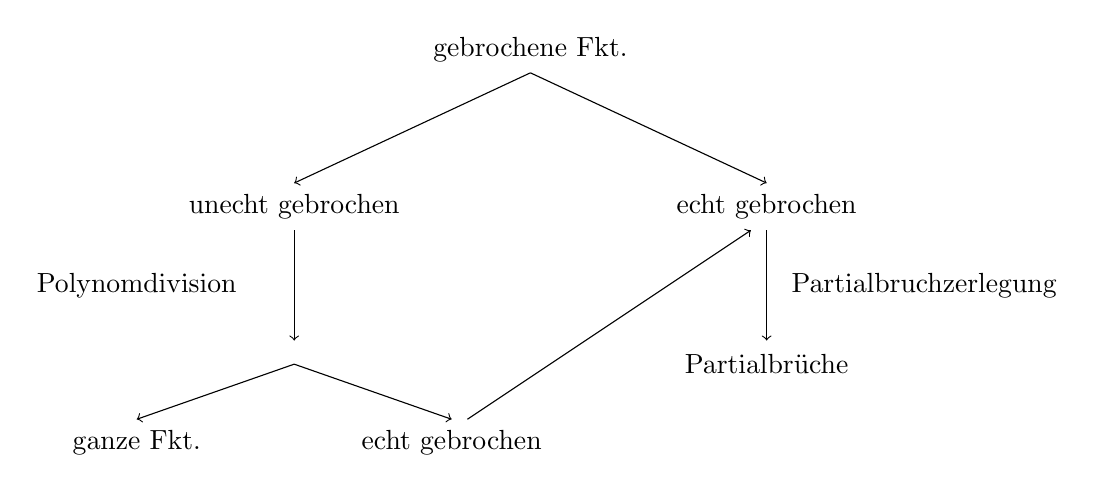
\begin{tikzpicture}
        \node[] at (0, 1) {gebrochene Fkt.};
        \node[] at (-3,-1) {unecht gebrochen};
        \node[] at (3,-1) {echt gebrochen};
        \node[] at (-5, -2) {Polynomdivision};
        \node[] at (-5, -4) {ganze Fkt.};
        \node[] at (-1, -4) {echt gebrochen};
        \node[] at (5, -2) {Partialbruchzerlegung}; 
        \node[] at (3, -3) {Partialbrüche}; 

        \draw[->] ( 0, 0.7) -- (-3,-0.7);
        \draw[->] ( 0, 0.7) -- ( 3,-0.7);
        \draw[->] (-3, -1.3) -- (-3,-2.7);
        \draw[->] (-3, -3)   -- (-5,-3.7);
        \draw[->] (-3, -3)   -- (-1,-3.7);
        
        \draw[->] (-0.8, -3.7) -- (2.8, -1.3);
        
        \draw[->] (3, -1.3) -- (3, -2.7);
    \end{tikzpicture}
    \caption{Umgang mit gebrochenen Funktionen}\label{fig:gebrochene_funktionen_graph}
\end{figure}

\subsubsection{Partialbruchzerlegung}

\[
    y = \frac{5x + 11}{x^2 + 3x - 10}    
\]

\paragraph{I.\;Prüfen: Wirklich echt gebrochen?}

\textit{Ja}

\paragraph{II.\;Nullstellen des Nenners}

\begin{gather*}
    x^2 + 3x - 10 = 0 \\
    x_{1,2} = -\frac{3}{2} \pm \sqrt{\frac{9}{4}+ \frac{40}{4}} = -\frac{3}{2} \pm \frac{7}{2} \\
    x_1 = 2 \quad x_2 = -5
\end{gather*}

\[
    \Rightarrow \frac{5x + 11}{(x-2)(x + 5)}
\]

\paragraph{III.\;Aufstellen der Partialbrüche}

\begin{align*}
    \frac{5x + 11}{(x-2)(x + 5)} &= \frac{A}{x - 2} + \frac{B}{x + 5} &&\mid \cdot ((x-2)(x+5)) \\
    5x + 11 &= A(x + 5) + B(x - 2)
\end{align*}

\paragraph{IV.\;Konstanten bestimmen}

Durch Einsetzen von Werten (Optimalerweise den Nullstellen):

\begin{align*}
    5x + 11 &= A(x + 5) + B(x - 2) \\
    \\
    x = 2:\\
    21 &= 7A  \Leftrightarrow A = \frac{21}{7} = 3 \\
    x = -5:\\
    -14 &= -7B \Leftrightarrow B = 2
\end{align*}

\paragraph{V.\;Einsetzen}

\[
    y = \frac{5x + 11}{x^2 + 3x - 10} = \frac{3}{x-2} + \frac{2}{x+5}  
\]

\paragraph{Anmerkung}

Die Partialbruchzerlegung ist ein Lösungsverfahren für Integrale, ist normalerweise nicht von Vorteil für
die Kurvendiskussion:

\[
    \int \frac{5x + 11}{x^2 + 3x - 10} \diff x = \int \frac{3}{x-2} \diff x + \int \frac{2}{x+5} \diff x 
\]

\paragraph{Fallunterscheidung}

\subparagraph{1. Fall}

\(N(x)\) hat nur einfache reelle Nullstellen, \(x_i\) sei eine dieser
Nullstellen.

Dann gehört zu \(x_i\) ein Partialbruch der Form:

\[
    \frac{A_i}{x - x_i}    
\]

\subparagraph{2. Fall}

\(N(x)\) hat an der Stelle \(x_i\) eine \(k\)-fache Nullstelle.

Dann gehören zu \(x_i\) \(k\) Partialbrüche der Form:

\[
    \frac{A_{i1}}{x - x_i}  + \frac{A_{i2}}{{(x - x_i)}^2} + \frac{A_{i3}}{{(x - x_i)}^3} + \cdots + \frac{A_{ik}}{{(x - x_i)}^k}   
\]

\subsubsection{Polynomdivision}

\[
	f(x) = x^3 + x^2 -8x - 12
\]

geschätzte Nullstelle: \(x_1 = 3\) \textrightarrow\ Polynomdivision:
\footnote{Aus technischen Gründen ist die Polynomdivision hier mit bereits aufgelösten Minusklammern dargestellt.}

\polyset{style=C, div=:,vars=x}
\polylongdiv{x^3 + x^2 -8x -12}{x -3}

\begin{uebung}
	Diskutieren Sie ohne Ableitung.

	\begin{question}
		\[
			y = \frac{x^3}{{(x-1)}^2}
		\]
	\end{question}

	\begin{solution}
		\[
			y = \frac{x^3}{{(x-1)}^2}
		\]

		\subparagraph{Nullstellen}
		Dreifache Nullstelle bei \(x = 0 \Rightarrow \) Sattelpunkt

		\subparagraph{Polstelle}
		Zweifache Polstelle bei \(x = 1 \Rightarrow \) PS ohne Vorzeichenwechsel

		\subparagraph{Symmetrie}
		weder gerade noch ungerade: nicht symmetrisch

		\subparagraph{Polynomdivision}
		\polyset{style=C, div=:,vars=x}
		\polylongdiv{x^3}{x^2 -2x + 1}

		\[
			y = \underbrace{x + 2}_{\text{\color{cyan}Asymptote}} + \underbrace{\frac{3x - 2}{{(x - 1)}^2}}_{\text{echt gebrochen}}
		\]

		\begin{figure}[H]
			\centering
			\begin{tikzpicture}
				\begin{axis}[
						default,
						xmin=-8.2, xmax=8.2,
						ymin=-8.2, ymax=8.2,
						width=8cm
					]
					\draw [color1, smooth, samples=100, domain=-8.2:0.9] plot (\x, {pow(\x, 3) / pow((\x - 1), 2)});
					\draw [color1, smooth, samples=100, domain=1.1:8.2] plot (\x, {pow(\x, 3) / pow((\x - 1), 2)});
					\draw [dashed, cyan, samples=100, domain=-8.2:8.2] plot (\x, {\x+2});
					\draw[dashed, gray] (1, -8.2) -- (1, 8.2);
				\end{axis}
			\end{tikzpicture}
			\caption{Skizze}
		\end{figure}
	\end{solution}

	\begin{question}
		\[
			y = x^3 + x^2 - 8x - 12
		\]
	\end{question}

	\begin{solution}
		\[
			y = x^3 + x^2 - 8x - 12
		\]

		\subparagraph{Nullstellen}
		1. Nullstelle raten: \(x_{N1} = 3\)

		\polyset{style=C, div=:,vars=x}
		\polylongdiv{x^3 + x^2 -8x -12}{x -3}

		2./3. Nullstelle bei \(x_{N2} = -2 \Rightarrow \) Extremwert (2-fache Nullstelle)

		\subparagraph{Symmetrie}
		weder gerade noch ungerade: nicht symmetrisch

		\[
			\limtoinfty{x} y = \infty; \limtomininfty{x} y = -\infty
		\]

		\begin{figure}[H]
			\centering
			\begin{tikzpicture}
				\begin{axis}[
						xmin=-8.2, xmax=8.2,
						ymin=-8.2, ymax=8.2,
						height=8cm,
						width=8cm,
						grid=both,
						axis lines=middle,
						grid style={line width=.1pt, draw=gray!20},
						major grid style={line width=.2pt,draw=gray!50},
						ticklabel style={font=\tiny},
						xlabel style={font=\tiny},
						ylabel style={font=\tiny},
						xlabel={x}, ylabel={y}
					]
					\draw [color1, smooth, samples=100, domain=-4:4] plot
					(\x, {pow(\x, 3) + pow(\x,2) - 8 * \x - 12});
				\end{axis}
			\end{tikzpicture}
			\caption{Skizze}
		\end{figure}
	\end{solution}
\end{uebung}


\subsection{Trigonometrische Funktionen}

\subsubsection{Herleitung am Einheitskreiss}

Der Einheitskreis wird beschrieben durch:

\[
	y^2+x^2 = 1
\]

oder auch

\[
	\sin^2(\alpha) + \cos^2(\alpha) = 1
\]

\begin{figure}[H]
	\centering
	\begin{tikzpicture}
		\begin{axis}[
				defaultnonumbers,
				xmin=-1.2, xmax=1.2,
				ymin=-1.2, ymax=1.2,
				width=8cm
			]
			\draw (1, 0) arc (0:360:1);
			\draw (0,0) -- (1.2, 1);
			\node at (axis cs: -1.1, 0.1) {1};
			\node at (axis cs: -0.1, -0.1) {M};
			\node at (axis cs: -0.1, 1.1) {D};
			\node at (axis cs: 1.1, -0.1) {B};
			\node at (axis cs: 0.9, 10/11) {C};
			\node at (axis cs: 0.6, 0.64) {P};
			\node at (axis cs: 0.77, -0.1) {A};
			\node at (axis cs: 1.1, 1.1) {E};
			\node at (axis cs: 0.2, 0.08) {\textalpha};
			\draw (0.3,0) arc (0:39.81:0.3);
			\draw[mkred, thick] (0,1) -- (1.2, 1);
			\node[mkred] at (axis cs: 0.5, 1.1) {cot(\textalpha)};
			\draw[mkgreen, thick] (0.77,0) -- (0.77, 0.64);
			\node[mkgreen, left] at (axis cs: 0.8, 0.25) {sin(\textalpha)};
			\draw[mkyellow, thick] (1,0) -- (1, 5/6);
			\node[mkyellow, rotate=90] at (axis cs: 1.1, 0.4) {tan(\textalpha)};
			\draw[mkblue, thick] (0,0) -- (0.77,0);
			\node[mkblue, below] at (axis cs: 0.4, 0) {cos(\textalpha)};
		\end{axis}
	\end{tikzpicture}
	\caption{Herleitung der trigonometrischen Funktionen am Einheitskreis}
\end{figure}

Die Funktionen:

\begin{itemize}
	\item {
	      \color{mkgreen}
	      \textbf{Sinus:}
	      }\\
	      \(\overline{PA} = \sin(\alpha)\)
	\item {
	      \color{mkblue}
	      \textbf{Cosinus\footnote{wird auch \enquote{Kosinus} geschrieben}:}
	      }\\
	      \(\overline{MA} = \cos(\alpha)\)
	\item {
	      \color{mkyellow}
	      \textbf{Tangens:}
	      }\\
	      \(\overline{BC} = \tan(\alpha)\)
	\item {
	      \color{mkred}
	      \textbf{Cotangens\footnote{wird auch \enquote{Kotangens} geschrieben}:}
	      }\\
	      \(\overline{DE} = \cot(\alpha)\)
\end{itemize}


\begin{align*}
	\frac{\sin(\alpha)}{\cos(\alpha)} & = \tan(\alpha) \\
	\frac{\cos(\alpha)}{\sin(\alpha)} & = \cot(\alpha)
\end{align*}

\subsubsection{Sinus \& Cosinus}

\begin{figure}[H]
    \centering
    \begin{tikzpicture}
        \begin{axis}[
            default,
            xmin=-1.2, xmax=7.2,
            ymin=-1.2, ymax=1.2,
            width=12cm
            ]
            \draw [mkgreen, smooth, samples=100, domain=-1.2:3*pi] plot (\x, {sin(\x r)});
            \draw [mkblue, smooth, samples=100, domain=-1.2:3*pi] plot (\x, {cos(\x r)});
            
            \draw[] (pi,-0.1) -- (pi,0.1);
            \node[] at (axis cs: pi, 0.3) {\(\pi\)};
            \draw[] (2*pi,-0.1) -- (2*pi,0.1);
            \node[] at (axis cs: 2*pi, 0.3) {\(2\pi\)};
        \end{axis}
    \end{tikzpicture}
    \caption{Sinus und Cosinus}
    \textbf{\color{mkgreen}---} \(\sin(x)\)
    \textbf{\color{mkblue}---} \(\cos(x)\)
\end{figure}

\begin{align*}
    \sin(-x) &= -\sin(x) &&\Rightarrow \text{punktsymmetrisch} \\
    \cos(-x) &= \cos(x) &&\Rightarrow \text{achsensymmetrisch} \\
    \\
    \sin(x + 2k \pi) &= \sin(x) &&k \in \mathbb{Z} \\
    \cos(x + 2k \pi) &= \cos(x) &&k \in \mathbb{Z} \\
\end{align*}

\begin{center}
    \(\sin(x)\) und \(\cos(x)\) sind periodisch mit \(2\pi \).
\end{center}

\subsubsection{Tangens \& Cotangens}

\begin{figure}[H]
    \centering
    \begin{tikzpicture}
        \tikzstyle{polstelle}=[dotted, thick]
        \begin{axis}[
            default,
            xmin=-1.2, xmax=7.2,
            ymin=-2.2, ymax=2.2,
            width=12cm
            ]
            \draw [mkyellow, smooth, samples=100, domain=-1.2:5/12*pi] plot (\x, {tan(\x r)});
            \draw [mkyellow, smooth, samples=100, domain=7/12*pi:17/12*pi] plot (\x, {tan(\x r)});
            \draw [mkyellow, smooth, samples=100, domain=19/12*pi:29/12*pi] plot (\x, {tan(\x r)});
            \draw [mkred, smooth, samples=100, domain=-11/12*pi:-1/12*pi] plot
            (\x, {cos(\x r) / sin(\x r)});
            \draw [mkred, smooth, samples=100, domain=1/12*pi:11/12*pi] plot
            (\x, {cos(\x r) / sin(\x r)});
            \draw [mkred, smooth, samples=100, domain=13/12*pi:23/12*pi] plot
            (\x, {cos(\x r) / sin(\x r)});
            \draw [mkred, smooth, samples=100, domain=25/12*pi:35/12*pi] plot
            (\x, {cos(\x r) / sin(\x r)});
            \draw[mkred, polstelle] (pi,-2.5) -- (pi,2.5);
            \draw[mkred, polstelle] (2*pi,-2.5) -- (2*pi,2.5);
            \draw[mkred, polstelle] (3*pi,-2.5) -- (3*pi,2.5);
            \draw[mkyellow, polstelle] (1/2*pi,-2.5) -- (1/2*pi,2.5);
            \draw[mkyellow, polstelle] (3/2*pi,-2.5) -- (3/2*pi,2.5);
            \draw[mkyellow, polstelle] (5/2*pi,-2.5) -- (5/2*pi,2.5);

            \draw[] (pi,-0.1) -- (pi,0.1);
            \node[] at (axis cs: pi, 0.3) {\(\pi\)};
            \draw[] (2*pi,-0.1) -- (2*pi,0.1);
            \node[] at (axis cs: 2*pi, 0.3) {\(2\pi\)};
        \end{axis}
    \end{tikzpicture}
    \caption{Tangens und Cotangens}
    \textbf{\color{mkyellow}---} \(\tan(x)\)
    \textbf{\color{mkred}---} \(\cot(x)\)
\end{figure}

\begin{align*}
    \tan(-x) &= -\tan(x) &&\Rightarrow \text{punktsymmetrisch} \\
    \cot(-x) &= -\cot(x) &&\Rightarrow \text{punktsymmetrisch} \\
    \\
    \tan(x + k \pi) &= \tan(x) &&k \in \mathbb{Z} \\
    \cot(x + k \pi) &= \cot(x) &&k \in \mathbb{Z} \\
\end{align*}

\begin{center}
    \(\tan(x)\) und \(\cot(x)\) sind periodisch mit \(\pi \).
\end{center}

\subsubsection{Überblick}

\begin{figure}[H]
    \centering
    \begin{tikzpicture}
        \tikzstyle{polstelle}=[dotted, thick]
        \begin{axis}[
            default,
            xmin=-0.2, xmax=8.2,
            ymin=-2.2, ymax=2.2,
            width=12cm
            ]
            \draw [mkgreen, smooth, samples=100, domain=-1:3*pi] plot (\x, {sin(\x r)});
            \draw [mkblue, smooth, samples=100, domain=-1:3*pi] plot (\x, {cos(\x r)});
            \draw [mkyellow, smooth, samples=100, domain=-1:5/12*pi] plot (\x, {tan(\x r)});
            \draw [mkyellow, smooth, samples=100, domain=7/12*pi:17/12*pi] plot (\x, {tan(\x r)});
            \draw [mkyellow, smooth, samples=100, domain=19/12*pi:29/12*pi] plot (\x, {tan(\x r)});
            \draw [mkred, smooth, samples=100, domain=1/12*pi:11/12*pi] plot
            (\x, {cos(\x r) / sin(\x r)});
            \draw [mkred, smooth, samples=100, domain=13/12*pi:23/12*pi] plot
            (\x, {cos(\x r) / sin(\x r)});
            \draw [mkred, smooth, samples=100, domain=25/12*pi:35/12*pi] plot
            (\x, {cos(\x r) / sin(\x r)});
            \draw[mkred, polstelle] (pi,-2.5) -- (pi,2.5);
            \draw[mkred, polstelle] (2*pi,-2.5) -- (2*pi,2.5);
            \draw[mkred, polstelle] (3*pi,-2.5) -- (3*pi,2.5);
            \draw[mkyellow, polstelle] (1/2*pi,-2.5) -- (1/2*pi,2.5);
            \draw[mkyellow, polstelle] (3/2*pi,-2.5) -- (3/2*pi,2.5);
            \draw[mkyellow, polstelle] (5/2*pi,-2.5) -- (5/2*pi,2.5);
            
            \draw[] (pi,-0.1) -- (pi,0.1);
            \node[] at (axis cs: pi, 0.3) {\(\pi\)};
            \draw[] (2*pi,-0.1) -- (2*pi,0.1);
            \node[] at (axis cs: 2*pi, 0.3) {\(2\pi\)};
        \end{axis}
    \end{tikzpicture}
    \caption{Die trigonometrischen Funktionen}
    \textbf{\color{mkgreen}---} \(\sin(x)\)
    \textbf{\color{mkblue}---} \(\cos(x)\)
    \textbf{\color{mkyellow}---} \(\tan(x)\)
    \textbf{\color{mkred}---} \(\cot(x)\)
\end{figure}



\begin{center}
    \begin{tabular}{ c c c c  } 
        Funktion & Definitionsbereich & Wertebereich & Symmetrie \\
        \toprule 
        \( \sin(x) \) & \( -\infty \leq x \leq \infty \) & \( -1 \leq y \leq 1
        \) & Punktsymmetrie \\
        \( \cos(x) \) & \( -\infty \leq x \leq \infty \) & \( -1 \leq y \leq 1
        \) & Achsensymmetrie \\
        \( \tan(x) \) & \( x \neq \frac{k}{2} \pi \) & \( -\infty \leq y \leq
        \infty \) & Punktsymmetrie \\
        \( \cot(x) \) & \( x \neq k \pi \) & \( -\infty \leq y \leq \infty \) &
        Punktsymmetrie \\
    \end{tabular}
\end{center}
    
    
\subsubsection{Rechenregeln}

\paragraph{Additionstheorem für Sinus}

\[
	\sin(\alpha + \beta) = \sin \alpha \cdot \cos \beta + \sin \beta \cdot \cos \alpha
\]

\begin{figure}[H]
	\centering
	\begin{tikzpicture}[font=\sffamily]
		\begin{axis}[
				defaultnonumbers,
				xmin=-0.2, xmax=1.2,
				ymin=-0.2, ymax=1.2,
				width=8cm,
				grid=none
			]
			\draw (1, 0) arc (0:360:1);

			% Strecke ME
			\draw (0,0) -- (1.2, 0.8);
			% Strecke MP
			\draw (0,0) -- (0.7, 1.1);

			% Winkel Alpha
			\draw[->] (0.4,0) arc (0:33.69:0.4);
			\node at (axis cs: 0.3, 0.08) {\textalpha};
			% Winkel Beta
			\draw[->] (0.33,0.22) arc (33.69:57.53:0.4);
			\node at (axis cs: 0.22, 0.22) {\textbeta};

			% Punktbeschriftung
			\node at (axis cs: 1.05, -0.1) {1};
			\node at (axis cs: -0.05, -0.05) {M};
			\node at (axis cs: 0.83, 0.65) {E};
			\node at (axis cs: 0.53, 0.9) {P};
			\node at (axis cs: 0.53, -0.05) {A};
			\node at (axis cs: 0.76, -0.05) {F};
			\node at (axis cs: 0.8, 0.45) {B};
			\node at (axis cs: 0.5, 0.5) {T};

			% Strecke AP
			\draw[mkred, thick] (0.54, 0) -- (0.54, 0.84);
			% Strecke PE
			\draw[mkblue, thick] (0.54, 0.84) -- (0.76, 0.5);
			% Rechter Winkel an B
			\draw[mkblue, thick] (0.71, 0.58) arc (123.69: 213: 0.085);
			\node[mkblue, thick] at (axis cs: 0.71, 0.51) {\( \cdot \)};
			% Strecke BF
			\draw[mkyellow, thick] (0.76, 0.5) -- (0.76, 0);
			% Strecke TB
			\draw[mkgreen, thick] (0.54, 0.5) -- (0.76, 0.5);
			% Markierung Strahlensatz 
			\draw[gray] (0.54, 0.42) -- (0.59, 0.39);
			\draw[gray] (0.49, 0.33) -- (0.54, 0.3);

			% Winkel Alpha an P
			\draw[->] (0.54, 0.7) arc (270: 303.69: 0.14);
			\node at (axis cs: 0.7, 0.8) {\textalpha};
			% Beschriftungslinie für Alpha
			\draw[thin] (0.56, 0.75) -- (0.67, 0.78);
		\end{axis}
	\end{tikzpicture}
	\caption{Herleitung des Additionstheorems}
\end{figure}


\[
	\underbrace{\sin(\alpha + \beta)}_{\overline{PA}} =
	\underbrace{\sin \alpha \cdot \cos \beta}_{\overline{AT}} +
	\underbrace{\sin \beta \cdot \cos \alpha}_{\overline{PT}}
\]

\begin{align*}
	\sin \alpha & = \frac{\overline{BF}}{\overline{MB}}
	            & \sin \beta                            & = \frac{\overline{PB}}{\overline{MP}} \\
	\cos \alpha & = \frac{\overline{PT}}{\overline{PB}}
	            & \cos \beta                            & = \frac{\overline{MB}}{\overline{MP}}
\end{align*}

\begin{align*}
	\sin \alpha = \frac{\overline{BF}}{\overline{MB}}
	\Leftrightarrow \overline{BF} = \sin \alpha \cdot \overline{MB}
	= \sin \alpha \cdot \cos \beta \\
	\cos \alpha = \frac{\overline{PT}}{\overline{PB}}
	\Leftrightarrow \overline{PT} = \cos \alpha \cdot \overline{PB}
	= \cos \alpha \cdot \sin \beta
\end{align*}

\paragraph{Beispiele}

\begin{align*}
	\sin(2 \alpha)
	 & = \sin\alpha \cdot \cos\alpha + \sin\alpha \cdot \cos\alpha    \\
	 & = 2 \cdot \sin\alpha \cdot \cos\alpha                          \\
	\\
	\cos(\alpha + \beta)
	 & = \sin\left(\alpha + \beta + \frac{\pi}{2}\right)              \\
	 & = \sin\left(\alpha + \left(\beta + \frac{\pi}{2}\right)\right) \\
	 & = \sin\alpha \cdot \cos\left( \beta + \frac{\pi}{2} \right)
	+ \sin\left( \beta + \frac{\pi}{2} \right) \cdot \cos\alpha       \\
	 & = \sin\alpha \cdot (-\sin\beta) + \cos\beta \cdot \cos\alpha   \\
	 & = \cos\alpha \cdot \cos\beta - \sin\alpha \cdot \sin\beta
\end{align*}

\subsubsection{Umkehrfunktionen}

\begin{figure}[H]
	\centering
	\begin{tikzpicture}[font=\sffamily]
		\begin{axis}[
				defaultnonumbers,
				xmin=-0.2, xmax=1.2,
				ymin=-0.2, ymax=1.2,
				width=8cm,
				xlabel={}, ylabel={}
			]
			\draw (1, 0) arc (0:360:1);
			\draw (0, 0) -- (1.2, 1);
			\node at (axis cs: -1.1, 0.1) {1};
			\node at (axis cs: -0.1, -0.1) {M};
			\node at (axis cs: 0.6, 0.64) {P};
			\node at (axis cs: 0.77, -0.1) {A};
			\node at (axis cs: 0.2, 0.08) {x};
			\draw (0.3,0) arc (0:39.81:0.3);

			\draw[mkblue, thick] (1, 0) arc (0:39.81:1);
			\node[mkblue, rotate=90] at (axis cs: 1.1, 0.25) {arcsin(x)};
			\draw[mkgreen, thick] (0.77,0) -- (0.77, 0.64);
			\node[mkgreen, left] at (axis cs: 0.8, 0.25) {sin(x)};
		\end{axis}
	\end{tikzpicture}
	\caption{Herleitung von \( \arcsin \) am Einheitskreis}
\end{figure}

\begin{figure}[H]
	\centering
	\begin{tikzpicture}[font=\sffamily]
		\begin{axis}[
				defaultnonumbers,
				xmin=-0.2, xmax=1.2,
				ymin=-0.2, ymax=1.2,
				width=8cm,
				xlabel={}, ylabel={}
			]
			\addplot [domain=-1:1, samples=100] ({cos(x)},{sin(x)});

			\draw (0,0) -- (1.2, 1);
			\node at (axis cs: -1.1, 0.1) {1};
			\node at (axis cs: -0.1, -0.1) {M};
			\node at (axis cs: 0.6, 0.64) {P};
			\node at (axis cs: 0.77, -0.1) {A};
			\node at (axis cs: 0.2, 0.08) {x};
			\draw (0.3,0) arc (0:39.81:0.3);

			\draw[mkred, thick] (1, 0) arc (0:39.81:1);
			\node[mkred, rotate=90] at (axis cs: 1.1, 0.25) {arccos(x)};
			\draw[mkgreen, thick] (0,0) -- (1, 0);
			\node[mkgreen] at (axis cs: 0.5, -0.1) {cos(x)};
		\end{axis}
	\end{tikzpicture}
	\caption{Herleitung von \( \arccos \) am Einheitskreis}
\end{figure}

\begin{gesetz}
	\begin{align*}
		\arcsin(x) + \arccos(x) = \frac{\pi}{2} \\
		\arctan(x) + \arccot(x) = \frac{\pi}{2}
	\end{align*}
\end{gesetz}

\begin{achtung}
	Auf dem Taschenrechner und auch in mancher Literatur findet sich die
	Schreibweise \( \arcsin = \sin^{-1} \), dass bedeutet jedoch nicht \(
	\frac{1}{\sin} \).
\end{achtung}

\begin{figure}[H]
	\centering
	\begin{tikzpicture}
		\tikzstyle{polstelle}=[dotted, thick]
		\begin{axis}[
				default,
				xmin=-2.2, xmax=4.2,
				ymin=-2.2, ymax=4.2,
				width=10cm,
				xtick distance=1,
				ytick distance=1,
				extra y tick style={grid=none},
				extra y ticks={pi, -pi/2, pi/2},
				extra y tick labels={\(\pi\),\(-\frac{\pi}{2}\),\(\frac{\pi}{2}\)}
			]
			\draw[mkyellow, very thin, smooth, samples=100, domain=-4.2:4.2]
			plot (\x, {sin(\x r)});

			\draw[mkred, very thin, smooth, samples=100, domain=-4.2:4.2]
			plot (\x, {cos(\x r)});

			\draw[mkblue, very thick, smooth, samples=100, domain=-1:1]
			plot (\x, {rad(asin(\x))});

			\draw[mkgreen, very thick, smooth, samples=100, domain=-1:1]
			plot (\x, {rad(acos(\x))});

			\draw[mkgreen, polstelle] (-2.2, pi) -- (4.2, pi);
			\draw[mkblue, polstelle] (-2.2, pi/2) -- (4.2, pi/2);
			\draw[mkblue, polstelle] (-2.2, -pi/2) -- (4.2, -pi/2);
		\end{axis}
	\end{tikzpicture}
	\caption{Die Umkehrfunktionen zu Sinus und Cosinus}
	\textbf{\color{mkblue}---} \(\arcsin(x)\)
	\textbf{\color{mkgreen}---} \(\arccos(x)\)
	\textbf{\color{mkyellow}---} \(\sin(x)\)
	\textbf{\color{mkred}---} \(\cos(x)\)
\end{figure}

\begin{figure}[H]
	\centering
	\begin{tikzpicture}
		\tikzstyle{polstelle}=[dotted, thick]
		\tikzstyle{standardfunktion}=[very thin]
		\begin{axis}[
				default,
				xmin=-4.2, xmax=4.2,
				ymin=-4.2, ymax=4.2,
				width=10cm,
				extra x tick style={grid=none},
				extra x ticks={-pi, pi},
				extra x tick labels={\(-\pi\),\(\pi\)},
				extra y tick style={grid=none},
				extra y ticks={pi, -pi/2, pi/2},
				extra y tick labels={\(\pi\),\(-\frac{\pi}{2}\),\(\frac{\pi}{2}\)}
			]
			\draw[mkyellow, standardfunktion, smooth, samples=100, domain=-4.2:-1.6]
			plot (\x, {tan(\x r)});
			\draw[mkyellow, standardfunktion, smooth, samples=100, domain=-1.4:1.4]
			plot (\x, {tan(\x r)});
			\draw[mkyellow, standardfunktion, smooth, samples=100, domain=1.6:4.2]
			plot (\x, {tan(\x r)});

			% \draw[mkyellow, polstelle] (-1/2*pi, -4.2) -- (-1/2*pi, 4.2);
			% \draw[mkyellow, polstelle] (1/2*pi, -4.2) -- (1/2*pi, 4.2);

			\draw[mkblue, very thick, smooth, samples=100, domain=-4.2:4.2]
			plot (\x, {rad(atan(\x)});

			\draw[mkgreen, very thick, smooth, samples=100, domain=-4.2:4.2]
			plot (\x, {rad(90-atan(\x))});

			\draw [mkred, standardfunktion, smooth, samples=100, domain=-4.2:-3.2]
			plot (\x, {cos(\x r) / sin(\x r)});
			\draw [mkred, standardfunktion, smooth, samples=100, domain=-3:-0.1]
			plot (\x, {cos(\x r) / sin(\x r)});
			\draw [mkred, standardfunktion, smooth, samples=100, domain=0.1:3]
			plot (\x, {cos(\x r) / sin(\x r)});
			\draw [mkred, standardfunktion, smooth, samples=100, domain=3.2:4.2]
			plot (\x, {cos(\x r) / sin(\x r)});

			% \draw[mkred, polstelle] (-pi, -4.2) -- (-pi, 4.2);
			% \draw[mkred, polstelle] (pi, -4.2) -- (pi, 4.2);

			% Vertikale Polstellen
			\draw[mkgreen, polstelle] (-4.2, pi) -- (4.2, pi);
			\draw[mkblue, polstelle] (-4.2, pi/2) -- (4.2, pi/2);
			\draw[mkblue, polstelle] (-4.2, -pi/2) -- (4.2, -pi/2);
		\end{axis}
	\end{tikzpicture}
	\caption{Die Umkehrfunktionen zu Tangens und Cotangens}
	\textbf{\color{mkblue}---} \(\arctan(x)\)
	\textbf{\color{mkgreen}---} \(\arccot(x)\)
	\textbf{\color{mkyellow}---} \(\tan(x)\)
	\textbf{\color{mkred}---} \(\cot(x)\)
\end{figure}

\begin{uebung}
	Vereinfachen.

	\begin{question}
		\[
			\frac{\sin(x)}{\cos(x)}
		\]
	\end{question}

	\begin{solution}
		\begin{align*}
			\frac{\sin(x)}{\cos(x)}                              \\
			 & = \frac{\tan(x) \cdot \cos(x)}{\tan(x)} = \cos(x)
		\end{align*}
	\end{solution}

	\begin{question}
		\[
			\frac{\cos(x)}{\cot(x)}
		\]
	\end{question}

	\begin{solution}
		\begin{align*}
			\frac{\cos(x)}{\cot(x)}                              \\
		 	& = \frac{\cos(x) \cdot \sin(x)}{\cos(x)} = \sin(x)
		\end{align*}
	\end{solution}

	\begin{question}
		\[
			\sqrt{1+ \tan^2(x)} \cdot \cos(x)
		\]
	\end{question}

	\begin{solution}
		\begin{align*}
			\sqrt{1+ \tan^2(x)} \cdot \cos(x)                                         \\
			 & = \sqrt{1 + \frac{\sin^2(x)}{\cos^2(x)}} \cdot \sqrt{\cos^2(x)}        \\
			 & = \sqrt{\left(1 + \frac{\sin^2(x)}{\cos^2{x}} \right) \cdot \cos^2(x)} \\
			 & = \sqrt{\cos^2(x) + \sin^2(x)} = \sqrt{1} = 1
		\end{align*}
	\end{solution}

	\begin{question}
		\[
			\sqrt{1 + \tan^2(x)} \cdot \cos(x)
		\]
	\end{question}

	\begin{solution}
		\begin{align*}
			\sqrt{1 + \tan^2(x)} \cdot \cos(x)   \\
			 & = (1 + \tan(x)) \cdot \cos(x)     \\
			 & = \cos(x) + \tan(x) \cdot \cos(x) \\
			 & = \cos(x) + \sin(x)
		\end{align*}
	\end{solution}
\end{uebung}


\subsection{Kegelschnitte}

\subsubsection{Allgemeine Form}

\[
	A x^2 + B y^2 + C x + D y + E = \sigma
\]

\subsubsection{Kreis}

\[
	A = B
\]

\begin{figure}[H]
	\centering
	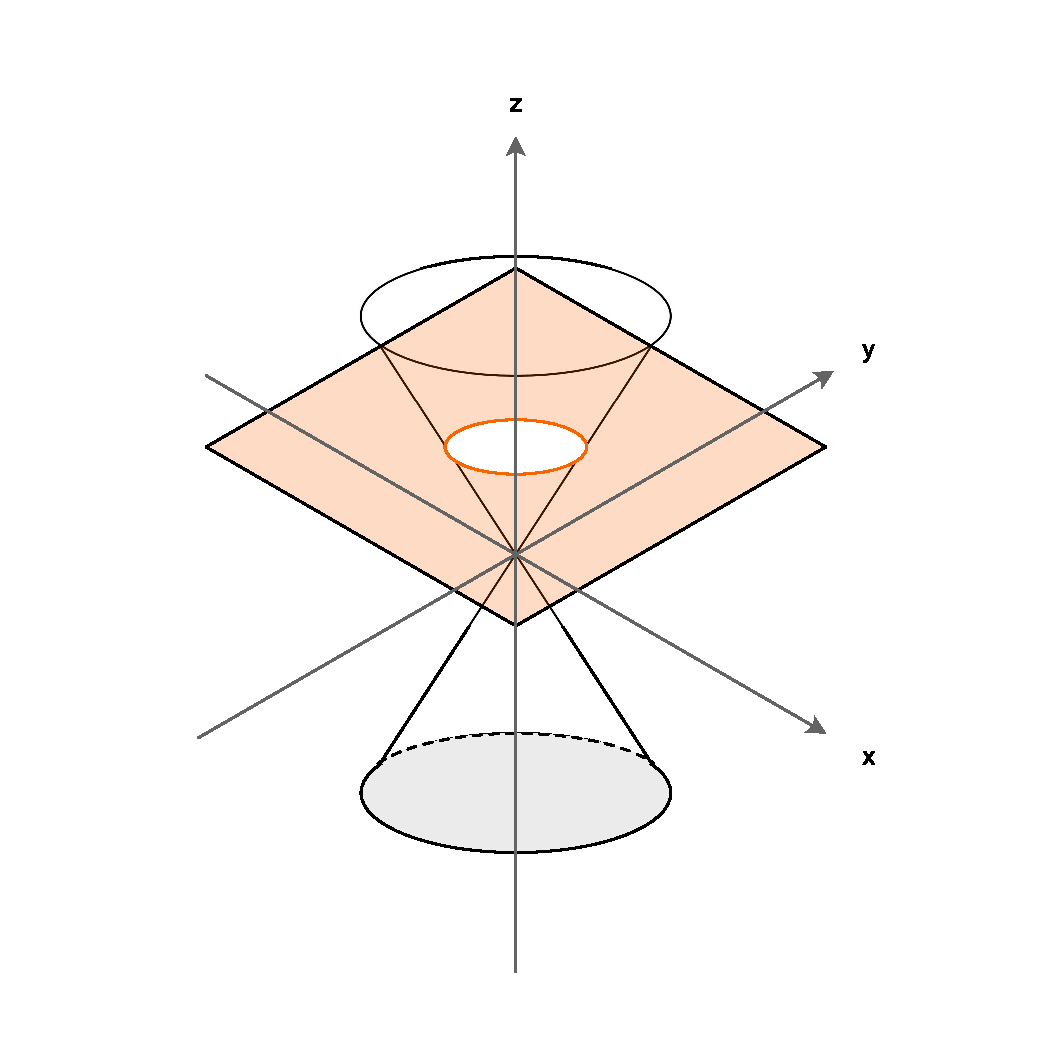
\includegraphics[width=8cm]{grafiken/kegelschnitte/kreis}
	\begin{tikzpicture}
		\begin{axis}[
				defaultnonumbers,
				xmin=-1.2, xmax=1.2,
				ymin=-1.2, ymax=1.2,
				width=8cm
			]
			\draw (0,0) ellipse [x radius=1, y radius=1];
		\end{axis}
	\end{tikzpicture}
	\caption{Kegelschnitt: Kreis}
\end{figure}

\paragraph{Einheitskreis}

\[
	A = B = 1 \quad E = -1 \quad x^2 + y^2 = 1
\]

\paragraph{Hauptform vom Kreis}

\[
	{(x - x_0)}^2 + {(y - y_0)}^2 = r^2
\]


\subsubsection{Ellipse}

\[
	A \cdot B > 0, A \neq B
\]

\begin{figure}[H]
	\centering
	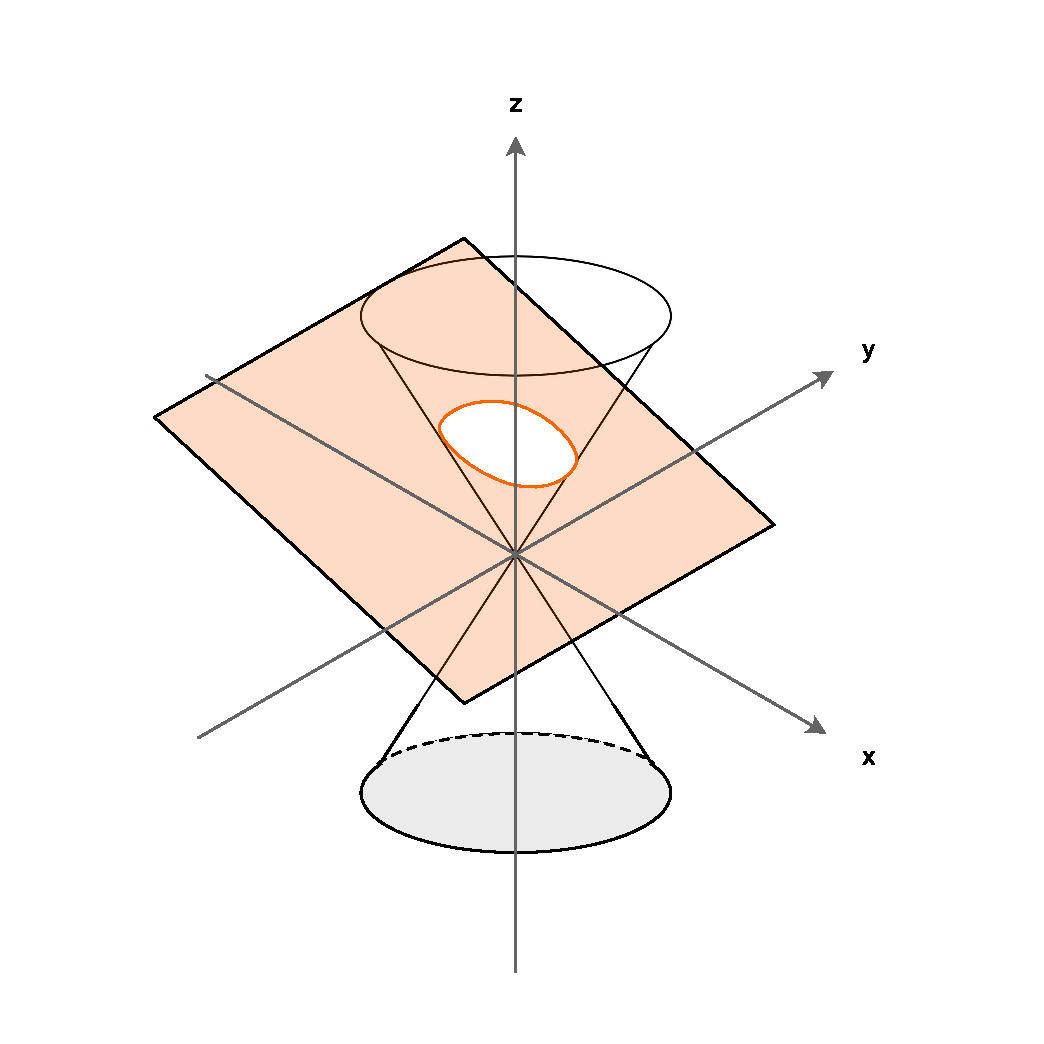
\includegraphics[width=8cm]{grafiken/kegelschnitte/ellipse}
	\begin{tikzpicture}
		\begin{axis}[
				defaultnonumbers,
				xmin=-2.2, xmax=2.2,
				ymin=-1.2, ymax=1.2,
				width=8cm
			]
			\draw (0,0) ellipse [x radius=2, y radius=1];
		\end{axis}
	\end{tikzpicture}
	\caption{Kegelschnitt: Ellipse}
\end{figure}

% \includegraphics{grafiken/Kegelschnitt_Ellipse}

\subsubsection{Hyperbel}

\[
	A \cdot B < 0, a \neq B
\]

\begin{figure}[H]
	\centering
	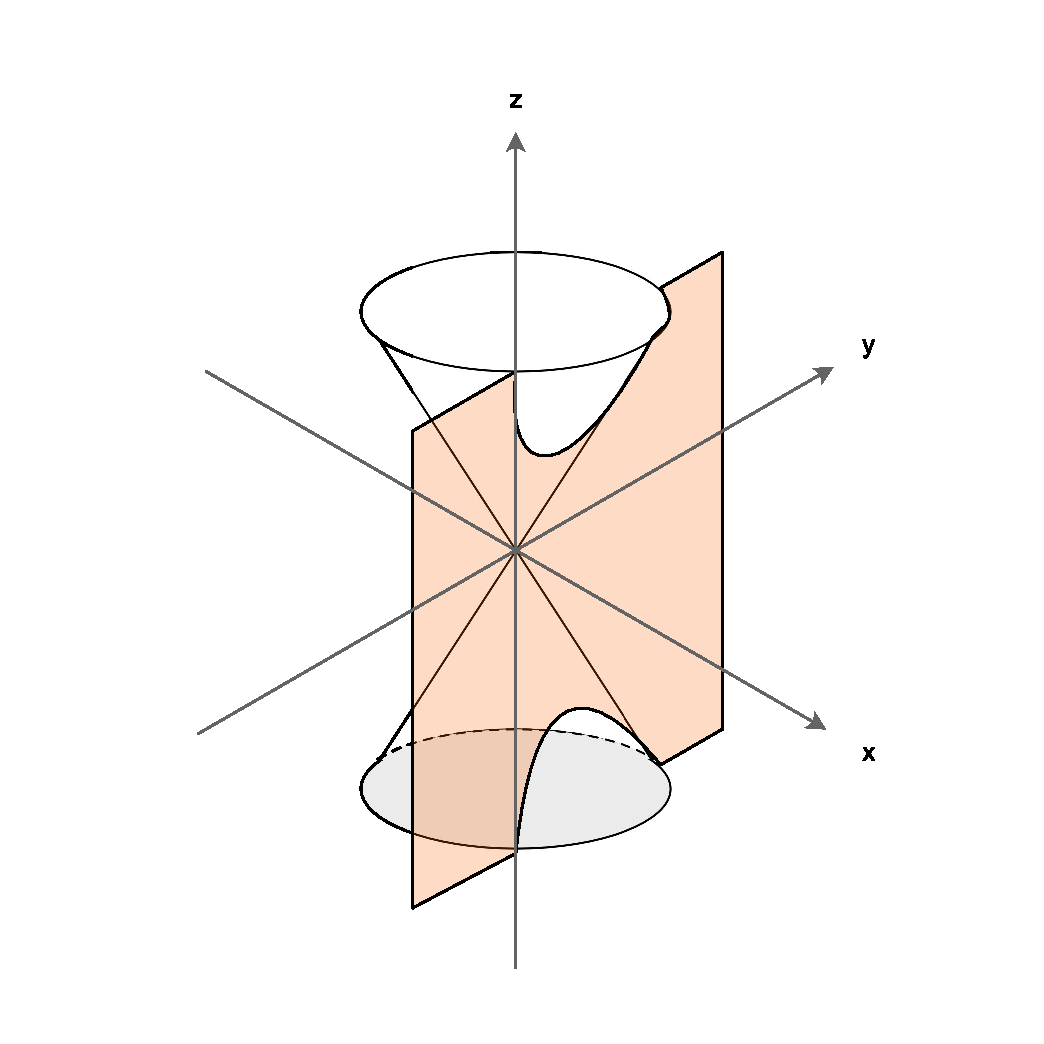
\includegraphics[width=8cm]{grafiken/kegelschnitte/hyperbel}
	\begin{tikzpicture}
		\begin{axis}[
				defaultnonumbers,
				xmin=-2.2, xmax=2.2,
				ymin=-2.2, ymax=2.2,
				width=8cm
			]
			\addplot [domain=-2:2] ({cosh(x)}, {sinh(x)});
			\addplot [domain=-2:2] ({-cosh(x)}, {sinh(x)});
		\end{axis}
	\end{tikzpicture}
	\caption{Kegelschnitt: Hyperbel}
\end{figure}

\subsubsection{Parabel}

\[
	(A = 0 \wedge B \neq 0) \vee (A \neq 0 \wedge B = 0)
\]

\begin{figure}[H]
	\centering
	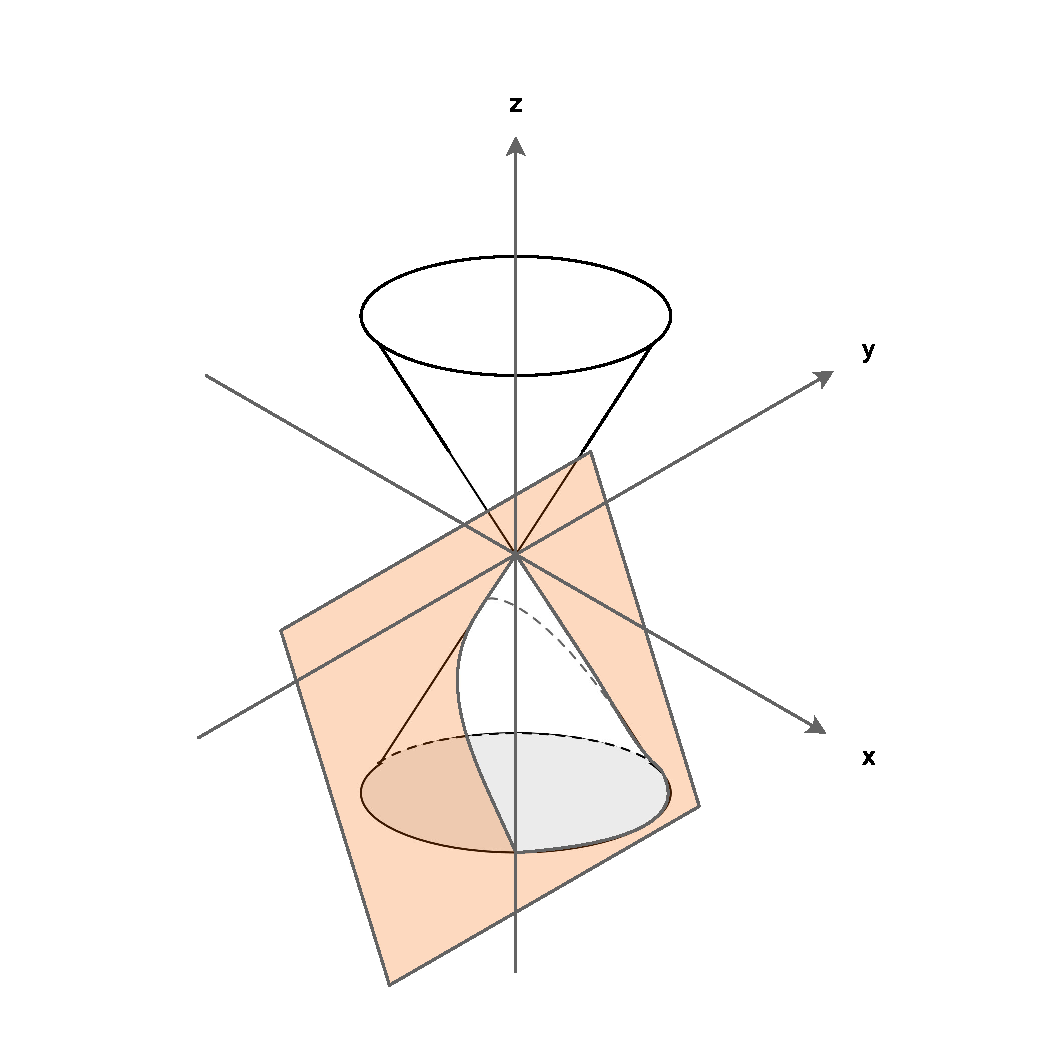
\includegraphics[width=8cm]{grafiken/kegelschnitte/parabel}
	\begin{tikzpicture}
		\begin{axis}[
				defaultnonumbers,
				xmin=-2.2, xmax=2.2,
				ymin=-2.2, ymax=2.2,
				width=8cm
			]
			\addplot [domain=-2:2] {x^2};
		\end{axis}
	\end{tikzpicture}
	\caption{Kegelschnitt: Parabel}
\end{figure}

\subsection{Exponentialfunktionen}

\paragraph{Allgemeine Form}

\[
	y = a^x \quad a \neq 1
\]

\begin{center}
	\( a > 0 \) damit wir in \( \mathbb{R} \) bleiben

	\( a \) wird Basis genannt, \( x \) Exponent

	\( a > 1 \) monoton steigend

	\( a < 1 \) monoton fallend
\end{center}

\begin{figure}[H]
	\centering
	\begin{tikzpicture}
		\begin{axis}[
				defaultnonumbers,
				xmin=-2.2, xmax=2.2,
				ymin=-1.2, ymax=3.2,
				width=8cm
			]
			\addplot[orange, smooth, samples=100, domain=-4:4] {e^x};
			\addplot[cyan, smooth, samples=100, domain=-4:4] {e^-x};
			\node [right] at (axis cs: 1.2, 3) {\( a > 1 \)};
			\node [left] at (axis cs: -1.2, 3) {\( a < 1 \)};
		\end{axis}
	\end{tikzpicture}
	\caption{exponentiell steigend (\( e^x \)) und fallend (\( e^{-x} \))}
\end{figure}

\begin{figure}[H]
	\centering
	\begin{align*}
		y(t)        & = {(1 + \omega)}^{t} \cdot y_0                            \\
		\Delta y(t) & \sim y(t-1)                                               \\
		\Delta y(t) & = \omega \cdot y(t-1) \quad \omega : \text{Wachstumsrate}
	\end{align*}
	\begin{tikzpicture}
		\begin{axis}[
				default,
				xmin=-1.2, xmax=6.2,
				ymin=-0.2, ymax=5.2,
				width=10cm,
				height=12cm,
				yticklabels={},
				xlabel={t},
			]
			\addplot [orange, smooth, samples=100, domain=-4:4] {e^(0.5*x)};

			\node [left] at (axis cs: -0.2, 1.0000) {\( y(0) \)};
			\node [left] at (axis cs: -0.2, 1.6487) {\( y(1) \)};
			\node [left] at (axis cs: -0.2, 2.7183) {\( y(2) \)};
			\node [left] at (axis cs: -0.2, 4.4817) {\( y(3) \)};

			\draw [dotted, thick] (-0.2, 1.0000) -- (6.2, 1);
			\draw [dotted, thick] (-0.2, 1.6487) -- (6.2, 1.6487);
			\draw [dotted, thick] (-0.2, 2.7183) -- (6.2, 2.7183);
			\draw [dotted, thick] (-0.2, 4.4817) -- (6.2, 4.4817);

			\draw [decorate,decoration={brace,amplitude=4pt}] (1, 1.6487) -- (1, 1);
			\draw [decorate,decoration={brace,amplitude=4pt}] (2, 2.7183) -- (2, 1.6487);
			\draw [decorate,decoration={brace,amplitude=4pt}] (3, 4.4817) -- (3, 2.7183);

			\node [right] at (axis cs: 1.2, 1.3244) {\( \Delta y(1) = \omega \cdot y(0) \)};
			\node [right] at (axis cs: 2.2, 2.1835) {\( \Delta y(2) = \omega \cdot y(1) \)};
			\node [right] at (axis cs: 3.2, 3.6000) {\( \Delta y(3) = \omega \cdot y(2) \)};
		\end{axis}
	\end{tikzpicture}
	\[
		\begin{alignedat}{5}
			\Delta y(3) &= y(3) - y(2) &= \omega \cdot y(2) \quad
			&\Rightarrow y(3) &= y(2) \cdot (1 + \omega) &= y(0) \cdot {(1+\omega)}^3 \\
			\Delta y(2) &= y(2) - y(1) &= \omega \cdot y(1) \quad
			&\Rightarrow y(2) &= y(1) \cdot (1 + \omega) &= y(0) \cdot {(1+\omega)}^2 \\
			\Delta y(1) &= y(1) - y(0) &= \omega \cdot y(0) \quad
			&\Rightarrow y(1) &= y(0) \cdot (1 + \omega) &= y(0) \cdot (1+\omega)
		\end{alignedat}
	\]
	% \caption{}
\end{figure}

\begin{uebung}[1]
	\begin{equation*}
		\begin{array}{lrl}
			                & 9^{x-1}       & = 27          \\
			\Leftrightarrow & 9^{x-1}       & = 3^3         \\
			\Leftrightarrow & {(3^2)}^{x-1} & = 3^3         \\
			\Leftrightarrow & 3^{2x-2}      & = 3^3         \\
			\Rightarrow     & 2x-2          & = 3           \\
			\Leftrightarrow & 2x            & = 5           \\
			\Leftrightarrow & x             & = \frac{5}{2}
		\end{array}
	\end{equation*}
\end{uebung}

\begin{uebung}[2]
	\begin{equation*}
		\begin{array}{lrl}
			                & {\left(\frac{4}{9}\right)}^{x-2}                    & = \frac{8}{27} \\
			\Leftrightarrow & {\left(\frac{4}{9}\right)}^{x-2}                    & =
			{\left(\frac{2}{3}\right)}^{3}                                                         \\
			\Leftrightarrow & {\left({\left(\frac{2}{3}\right)}^{2}\right)}^{x-2} & =
			{\left(\frac{2}{3}\right)}^{3}                                                         \\
			\Leftrightarrow & {\left(\frac{2}{3}\right)}^{2x-4}                   & =
			{\left(\frac{2}{3}\right)}^{3}                                                         \\
			\Rightarrow     & 2x-4                                                & = 3            \\
			\Leftrightarrow & 2x                                                  & = 7            \\
			\Leftrightarrow & x                                                   & = \frac{7}{2}
		\end{array}
	\end{equation*}
\end{uebung}

\begin{uebung}[3]
	\begin{equation*}
		\begin{array}{lrlr}
			                & 8 \cdot 9^{x-3} + 4^{x-3}     & = 3^{2x-4}                                    &                            \\
			\Leftrightarrow & 8 \cdot 3^{2x-9} + 4^{x-3}    & = 3^{2x-4}                                    &                            \\
			\Leftrightarrow & 2^3 \cdot 3^{2x-9} + 2^{2x-6} & = 3^{2x-4}                                    & \mid -(2^3 \cdot 3^{2x-9}) \\
			\Leftrightarrow & 2^{2x-6}                      & = 3^{2x-4} - 2^3 \cdot 3^{2x-9}               &                            \\
			\Leftrightarrow & 2^{2x-6}                      & = 3^{2} \cdot 3^{2x-6} - 2^{3} \cdot 3^{2x-9}                              \\
			\Leftrightarrow & 2^{2x-6}                      & = (3^2 - 2^3)
			% TODO: siehe Zettel - ergänzen 
		\end{array}
	\end{equation*}
\end{uebung}

\subsection{Logarithmusfunktionen}

Die Lösung \( x \) der Gleichung \( a^x = b \) nennt man
den Logarithmus von \( b \) zur Basis \( a \):

\[
    x = \log_a(b)
\]

Der Logarithmus von \( b \) zur Basis \( a \) ist jene reelle
Zahl \( x \) mit der man \( a \) potenzieren muss, um \( b \)
zu erhalten:

\[
    a^{\log_a(b)} = b    
\]

Die Logarithmusfunktion ist damit die Umkehrfunktion zur
Exponentialfunktion.


\begin{figure}[H]
    \centering
    \begin{tikzpicture}
        \begin{axis}[
                default,
                xmin=-2.2, xmax=2.2,
                ymin=-1.2, ymax=3.2,
                width=8cm
            ]
            \addplot[orange, smooth, samples=100, domain=0:2.2] {ln(x)};
            \addplot[cyan, smooth, samples=100, domain=0:2.2] {-ln(x)};
        \end{axis}
    \end{tikzpicture}
    \caption{Logarithmus steigend (\( \ln(x) \)) und fallend (\( -\ln{x} \))}
\end{figure}


\paragraph{Basis:}
\begin{equation*}
    \begin{array}{lll}
        a = e &\Rightarrow \log_e(x) &= \ln(x) \\
        a = 2 &\Rightarrow \log_2(x) &= \ld(x) = \lb(x) \\
        a = 10 &\Rightarrow \log_{10}(x) &= \lg(x)
    \end{array}
\end{equation*}

\subsubsection{Rechenregeln}

\begin{align*}
    \ln(a \cdot b) &= \ln(e^{\alpha} \cdot e^{\beta}) \\
    &= \ln(e^{(\alpha + \beta)}) \\
    &= \alpha + \beta \\
    &= \ln(e^{\alpha}) + \ln(e^{\beta}) \\
    &= \ln(a) + \ln (b) \\
    \\
    \ln(a^3) &= \ln(a^2 \cdot a) \\
    &= \ln(a^2) + \ln(a) \\
    &= \ln(a) + \ln(a) + \ln(a) \\
    &= 3 \cdot \ln(a) \\
    \\
    \ln(a^n) &= n \cdot \ln(a) \\
    \\
    \ln(\frac{a}{b}) &= \ln(a) + \ln(b^{-1}) \\
    &= \ln(a) - \ln(b)
\end{align*}

\subsubsection{Basiswechsel}
\[
    \log_a(x) \rightarrow \log_b(x)    
\]

\begin{align*}
    \log_a(x) = \log_a\left(b^{\log_b(x)}\right)
    &= \log_b(x) \cdot \log_a(b) \\
    \Rightarrow \log_a(x) &= \log_b(x) \cdot \frac{1}{\log_b(a)} \\
    \Rightarrow \log_a(x) &= \frac{\log_b(x)}{\log_b(a)} \\
    \text{wenn \(x = a\):} \\
    \log_a(a) &= \log_b(a) \cdot \log_a(b) = 1 \\
    \Rightarrow \log_a(b) &= \frac{1}{\log_b(a)} \\
    \\
    \text{Beispiel:} \\
    \log_3(5) &= \frac{\ln(5)}{\ln(3)}
\end{align*}

\paragraph{Beispiele}

\begin{align*}
    & \log(2) - \log(a) + \frac{1}{2} \log(b) \\
    &= \log\left(\frac{2}{a}\right) + \log\left(b^{\frac{1}{2}}\right) \\
    &= \log\left(\frac{2}{a}\right) + \log\left(\sqrt{b}\right) \\
    &= \log\left(\frac{2 \sqrt{b}}{a}\right)
\end{align*}

\begin{align*}
    \log(1-x) + \log(1+x) - 2 \log(x) \\
    &= \log((1-x)(1+x)) - \log\left(x^2\right) \\
    &= \log(1-x^2) - \log\left(x^2\right) \\
    &= \log\left(\frac{1-x^2}{x^2}\right) = \log\left(\frac{1}{x^2}-1\right)
\end{align*}

\begin{align*}
    10^x &= 2 \\
    \lg\left(10^x\right) &= \lg(2) \\
    x \lg(10) &= \lg(2) \\
    x \cdot 1 &= \lg(2) \\
    x &= \lg(2)
\end{align*}

\subsection{Stetigkeit und Grenzwert von Funktionen}

\[
	\lim_{x \rightarrow x_0} f(x) = g
\]

\( f(x) \) hat an der Stelle \( x_0 \) den Grenzwert \( g \),
wenn es zu einem beliebig kleinen \( \epsilon > 0 \) eine Zahl \( \delta(\epsilon) \)
gibt, so dass \( \mid f(x) - g \mid < \epsilon \) ist,
\( \forall x \) für die \( \mid x - x_0 \mid < \delta \) gibt.

\begin{figure}[H]
	\centering
	\begin{tikzpicture}
		\begin{axis}[
				default,
				xmin=-2.5, xmax=3.5,
				ymin=-0.5, ymax=3.5,
				width=8cm,
				xticklabels={},
				yticklabels={}
			]
			\addplot[color1, smooth, samples=100, domain=-4:4] {1.5^x};

			\draw [dotted, thick] (1, -0.2) -- (1, 1.5);
			\draw [dotted, thick] (2, -0.2) -- (2, 2.25);
			\draw [dotted, thick] (3, -0.2) -- (3, 3.375);

			\draw [dotted, thick] (-0.2, 1.5) -- (1, 1.5);
			\draw [dotted, thick] (-0.2, 2.25) -- (2, 2.25);
			\draw [dotted, thick] (-0.2, 3.375) -- (3, 3.375);

			\node at (axis cs: 1, -0.3) {\( x_0 - \delta \)};
			\node at (axis cs: 2, -0.3) {\( x_0 \)};
			\node at (axis cs: 3, -0.3) {\( x_0 + \delta \)};

			\node[left] at (axis cs: -0.2, 1.5) {\( y_0 - \epsilon \)};
			\node[left] at (axis cs: -0.2, 2.25) {\( f(x_0) = y_0 \)};
			\node[left] at (axis cs: -0.2, 3.375) {\( y_0 + \epsilon \)};
		\end{axis}
	\end{tikzpicture}
	\caption{}
\end{figure}

\subsubsection{Definitionslücke}

\paragraph{Beispiel}

\[
	y = \frac{x^2 - 1}{x - 1}
\]

\begin{figure}[H]
	\centering
	\begin{tikzpicture}
		\begin{axis}[
				default,
				xmin=-0.5, xmax=3.5,
				ymin=-0.5, ymax=3.5,
				width=8cm
			]
			\addplot[orange, smooth, samples=100, domain=-4:4] {(x^2 - 1) / (x - 1)};
			\addplot[mark=o] coordinates {(1,2)};
			\node[right] at (axis cs: 1, 2) {Definitionslücke};
		\end{axis}
	\end{tikzpicture}
	\caption{\(\frac{x^2 - 1}{x - 1}\)}
\end{figure}

\[
	\lim_{x \rightarrow 1} \frac{x^2 - 1^2}{x - 1}
	= \lim_{x \rightarrow 1} \frac{(x - 1)(x + 1)}{x - 1}
	= \lim_{x \rightarrow 1} (x+1)
	= 2
\]

\textbf{rechtseitiger Grenzwert}

\[
	x > x_0: \lim_{x \rightarrow x_0} f(x) = 2 = g_{+}
\]

\textbf{rechtseitiger Grenzwert}

\[
	x < x_0: \lim_{x \rightarrow x_0} f(x) = 2 = g_{-}
\]


\[
	g_{+} = g_{-} \Rightarrow \text{\(f(x_0)\) ist nicht definiert}
\]

\subsubsection{Sprungstelle}

\begin{figure}[H]
    \centering
    \begin{tikzpicture}
        \begin{axis}[
                default,
                xmin=-0.5, xmax=3.5,
                ymin=-0.5, ymax=3.5,
                width=8cm,
                xticklabels={},
                yticklabels={}
            ]
            \addplot[orange, smooth, samples=100, domain=-4:2] {2^x - 2};
            \addplot[orange, smooth, samples=100, domain=2:4] {-(x - 2)^2 + 3};
            
            \draw [dotted, thick] (2, -0.2) -- (2, 3.2);
            \node at (axis cs: 2, -0.3) {Sprungstelle};
        \end{axis}
    \end{tikzpicture}
    \caption{Funktion mit Sprungstelle}
\end{figure}

\[
    f(x) = 
    \begin{cases}
        2^x - 2 &\quad x \leq 2 \\
        -(x - 2)^2 + 3 &\quad x > 2
    \end{cases}
\]

\[
    g_{+} \neq g_{-} \Rightarrow \text{Sprungstelle}
\]

\subsubsection{Polstelle}

\begin{figure}[H]
    \centering
    \begin{tikzpicture}
        \begin{axis}[
                default,
                xmin=-2.5, xmax=2.5,
                ymin=-2.5, ymax=2.5,
                width=8cm
            ]
            \addplot[orange, smooth, samples=100, domain=-4:-0.1] {1/x};
            \addplot[orange, smooth, samples=100, domain=0.1:4] {1/x};
        \end{axis}
    \end{tikzpicture}
    \caption{\(y = \frac{1}{x}\)}
\end{figure}

\begin{align*}
    \begin{rcases}
        \lim_{x \rightarrow 0_+} f(x) &= \infty \\
        \lim_{x \rightarrow 0_-} f(x) &= -\infty
    \end{rcases}
    f(x), g\; \text{existieren nicht}
\end{align*}


